%\AddToShipoutPictureBG{%
%\begin{tikzpicture}[remember picture, overlay]
%\node[opacity=.9, inner sep=0pt]
%\vspace{3cm}
%    at(current page.center){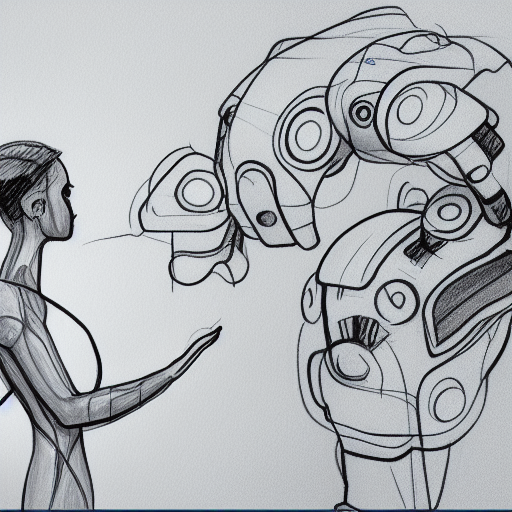
\includegraphics[width=22cm, height=30cm]{cover}};
%\end{tikzpicture}%
%}

\makeatletter         
\def\@maketitle{
% \includegraphics[scale=1, height=2.2cm]{figures/brdx.pdf}
% \hfill
% \vspace{-0.3cm}
% \includegraphics[scale=1, height=1.7cm]{figures/dga.png}
% \hfill
% \includegraphics[scale=1, height=2.cm]{figures/inria.png}
% \thispagestyle{empty}
% \begin{changemargin2}{-0.1cm}{-0.1cm}
\begin{center}
    {

    
\includegraphics[scale=1, height=1.5cm]{figures/logos.png}
    \DoubleSpacing
    \begin{large}
        \vspace{.55cm}


        {\huge \textbf{Towards Interactive Social Artificial Agents}} \\     
        % \vspace{0.15cm}
        {\Large \textbf{Formation and Exploitation of Cultural Conventions in Autonomous Embodied Artificial Agents\\}}
        
        \vspace{0.5cm}
        
        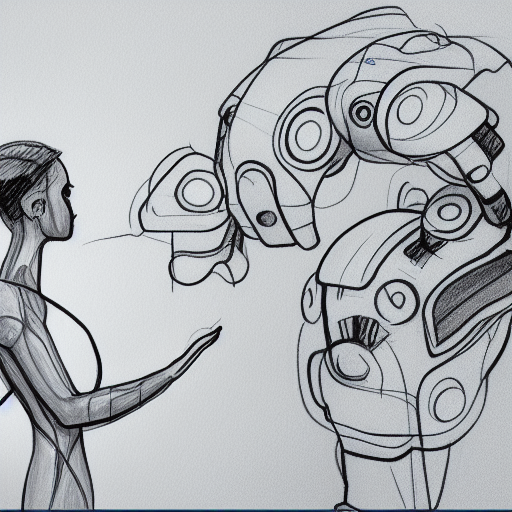
\includegraphics[width=7cm]{cover}
        
        \rule{0.2\textwidth}{0.6pt}
        
        {\Large By \textbf{Tristan Karch} \\}
        
        \vspace{0.5cm}

        \begin{normalsize}
            Under the supervision of Pierre-Yves Oudeyer \& Clément Moulin-Frier \\
            \vspace{0.5cm}
            In partial fulfillment of the requirements\\
            for the degree of Doctor of Philosophy \\
            
            \rule{0.05\textwidth}{0.4pt}

            University of Bordeaux \\
            Graduate school of Mathematics and Computer Science \\
            Major in Computer Science \\
        \end{normalsize}
    
        \rule{0.2\textwidth}{0.6pt}
        % UNIVERSITY OF BORDEAUX \\
        % GRADUATE SCHOOL OF MATHEMATICS AND COMPUTER SCIENCE\\
        % {\normalsize COMPUTER SCIENCE SPECIALTY} \\

    \end{large}
    }
\end{center}

\begin{small}
    
\noindent Submitted on X. Defended on Y.
\vfill
\noindent Composition of the jury:

%\begin{table}[b]
%\centering
%\resizebox{1.1\textwidth}{!}{%
%\hspace{-1.5cm}
%\begin{tabular}{lllr}
%Dr. X Y & Position & Affiliation & Reviewer / Examinator \\
%
%\end{tabular}
%}
%\end{table}
\end{small}

% \end{changemargin2}

}

